\documentclass[a4paper,6pt]{extarticle}
\usepackage[utf8]{inputenc}
\usepackage[landscape,top=0.6cm,bottom=0.6cm,left=0.6cm,right=0.6cm]{geometry}
\usepackage{amsmath}
\usepackage{amssymb}
\usepackage{multicol}
\usepackage{enumitem}
\usepackage{xcolor}
\usepackage{titlesec}
\usepackage{tikz}
\usetikzlibrary{shapes.geometric, arrows, positioning}

\setlength{\parindent}{0pt}
\setlength{\parskip}{0.2pt}
\setlength{\columnsep}{0.3cm}
\setlist{nosep,leftmargin=*,itemsep=0pt}
\titlespacing*{\section}{0pt}{1pt}{0.2pt}
\titlespacing*{\subsection}{0pt}{0.8pt}{0.2pt}
\titleformat*{\section}{\small\bfseries\color{blue}}
\titleformat*{\subsection}{\footnotesize\bfseries\color{red}}

\pagestyle{empty}

\begin{document}

\begin{multicols}{3}
\footnotesize

\section*{RF SYSTEMS}

\subsection*{Antennas: Gain \& Beamwidth}
$$G = \eta \left(\frac{\pi d f}{c}\right)^2 \quad G_{dBi} = 10\log_{10}(G) \quad A_e = \frac{G \lambda^2}{4\pi}$$
$$\boxed{\theta_{3dB} \approx \frac{70\lambda}{d} = \frac{70c}{fd} = \frac{21}{d_{\text{m}} f_{\text{GHz}}}} \text{ [deg]}$$
$\eta$ = 0.5-0.7 • Smaller $d$ → wider beam

\subsection*{FSL - Free Space Loss}
$$\boxed{A_{FSL} = 32.45 + 20\log(d_{km}) + 20\log(f_{MHz})} \text{ [dB]}$$
$$\boxed{A_{FSL} = 92.45 + 20\log(d_{km}) + 20\log(f_{GHz})} \text{ [dB]}$$
$2\times d$ → +6dB • $2\times f$ → +6dB • 60dB MHz/GHz

\subsection*{Propagation Losses}
$$\boxed{A_{total} = A_{FSL} + A_{atm} + A_{rain} + A_{pol} + A_{point}}$$
$A_{atm} = \alpha_{atm} \cdot d$ • $A_{rain} = \alpha_R L_{eff}$, $L_{eff} = h_R/\sin\varepsilon$
$A_{pol} = -20\log|\cos\Delta\theta|$ • $A_{point} \approx 12(\theta_{err}/\theta_{3dB})^2$

\subsection*{Link Budget}
$$\text{EIRP} = P_{TX} + G_{TX} \quad P_R = \text{EIRP} + G_{RX} - A_{total}$$
$$C/N = P_R - N \quad P_{sens} = N + (C/N)_{req}$$
Margin: $M = P_R - P_{sens}$ (min 2-3 dB) • Multi-hop: $\frac{1}{(C/N)_{tot}} = \sum \frac{1}{(C/N)_i}$

\subsection*{Noise - Friis Formula}
$$\boxed{F_{tot} = F_1 + \frac{F_2-1}{G_1} + \frac{F_3-1}{G_1 G_2} + \cdots} \text{ [LINEAR!]}$$
$F = 10^{F_{dB}/10}$, $G = 10^{G_{dB}/10}$ • Passive: $F = L$, $G = 1/L$
$$T_{eq} = T_0(F-1) \quad N = kT_{tot}B \quad k = 1.38 \times 10^{-23}$$
$$N_{dBm} = -174 + 10\log(T/290) + 10\log(B_{Hz})$$
$T_A$: Earth 260-290K, Sky 30-50K, Rain 260-280K, Space 5-10K

\subsection*{PA \& Modulation}
$P_{nom} = P_{1dB} - BO$ • PAPR: QPSK 3dB, 16QAM 4-5dB, OFDM 10-12dB
\textbf{C/N req (BER $10^{-3}$):} BPSK 6-9dB, QPSK 10-13dB, 16QAM 16-20dB, 64QAM 24-28dB, 256QAM 32-36dB
\textbf{Spectral Eff:} BPSK 1bit/s/Hz, QPSK 2, 16QAM 4, 64QAM 6, 256QAM 8
$R_b = B \times \log_2(M)$ • $E_b/N_0 = (C/N) \times (B/R_b)$ • Shannon: $C = B\log_2(1+C/N)$

\subsection*{Satellite Links}
\textbf{Orbits:} LEO 500-2000km, MEO 2000-35786km, GEO 35786km
\textbf{Doppler:} $\Delta f = f_0 (v/c) \cos\theta$ • LEO: $\pm$40kHz @ 2GHz
\textbf{Delay:} LEO 3-10ms, MEO 50-150ms, GEO 250-280ms (RT: ×2)
$G/T$ (G°K$^{-1}$): Quality factor • $G/T = G_{dBi} - 10\log(T_{sys})$

\section*{OPTICAL SYSTEMS}

\subsection*{Line Rate \& Spectral Efficiency}
$$R_{line} = N_{pol} \times R_s \times \log_2(M) \times FEC \quad R_{PL} = R_{line}/(1+OH)$$
$$\eta = \frac{R_{PL}}{B_{ch}} \text{ [bit/s/Hz]} \quad B_{ch} = R_s(1+\beta), \beta \approx 0.1\text{-}0.3$$
DP-QPSK: $4R_s$ • DP-16QAM: $8R_s$ • Shannon: $C = B\log_2(1+OSNR)$

\subsection*{OSNR}
$$OSNR_{dB} = P_{ch} - 10\log(P_{ASE,tot}) \quad B_{opt} = 12.5 \text{ GHz}$$
$$\boxed{OSNR = P_{ch} - F_{dB} - 58 - 10\log(N_{amp})} \text{ [dB, C-band]}$$
$P_{ASE,tot} = N_{amp} \times P_{ASE,1amp}$ • Margin: $OSNR \geq OSNR_{th} + 2$dB

\subsection*{ASE Noise}
$$P_{ASE} = 2n_{sp}h\nu(G-1)B_{opt} \approx 2n_{sp}h\nu GB_{opt}$$
$$P_{ASE} \approx 5.1 \times 10^{-9} G \text{ [W]} \quad P_{ASE,dBm} = -58 + F_{dB}$$
$F = 2n_{sp}$ • EDFA: $F = 4\text{-}6$dB → $n_{sp} = 1.3\text{-}2.0$
Const: $h = 6.626 \times 10^{-34}$, $\nu = 194$THz, $2h\nu B_{opt} = 4.96 \times 10^{-9}$W

\subsection*{Link Engineering}
$N_{amp} = \lceil L/D_{amp}\rceil - 1$ • $D_{amp} = G_{max}/\alpha$ • $\alpha \approx 0.18$dB/km
$$N_{ch} = \lfloor B_{amp}/\Delta f\rfloor \quad P_{ch} = P_{out} - 10\log(N_{ch})$$
Design: (1) $N_{amp}$ (2) $N_{ch}$ (3) $P_{ch}$ (4) Check OSNR (5) $C = N_{ch} \times R_{PL}$
\textbf{Dispersion:} $D \approx 17$ ps/(nm·km) @ 1550nm • Comp: DCF, DSP
\textbf{Nonlinear:} SPM, XPM, FWM • Limit: $P_{ch} < -3$dBm (high power)

\subsection*{Unamplified Budget}
$$Budget = P_{TX} - P_{RX,sens} - L_{conn} - L_{MUX} \quad L_{max} = Budget/\alpha$$
Losses: Fiber 0.18-0.20dB/km, Conn 0.3-0.5dB, Patch 0.5-0.6dB, MUX 5dB(40ch), 6dB(80ch)
\textbf{Splices:} 0.05-0.1dB/splice • \textbf{Bending:} $>$R$_{min}$ (typ 30mm)
\textbf{P2P Metro:} Typ 50-80km unamp • With boost+preamp: 80-120km

\subsection*{OSNR Required (BER $10^{-3}$)}
DP-QPSK: 10-13dB • DP-8QAM: 15-17dB • DP-16QAM: 19-22dB • DP-64QAM: 27-30dB

\subsection*{Fiber Types}
\textbf{SMF (G.652):} $\alpha$=0.18-0.20dB/km, D=17ps/(nm·km), Core 9μm
\textbf{NZDSF (G.655):} D=2-6ps/(nm·km) • \textbf{DCF:} D=-80 to -100ps/(nm·km)
\textbf{MMF:} Core 50/62.5μm, short dist (<2km), $\alpha$=2-3dB/km

\section*{ARCHITECTURES}

\subsection*{Receivers}
\textbf{Superheterodyne:} $f_{IF} = |f_{RF} - f_{LO}|$, $f_{LO} = f_{RF} \pm f_{IF}$
$f_{image} = f_{LO} + f_{IF}$ • Pros: selectivity • Cons: image problem
\textbf{Homodyne:} $f_{LO} = f_{RF}$, $f_{IF} = 0$ • Pros: simple, no image • Cons: DC offset

\subsection*{Coherent Optical}
Pros: amp+phase, dual-pol ($\times$2), DSP, sens↑, $\eta > 4$

\subsection*{WDM}
$N_{ch} = \lfloor B_{amp}/(\Delta f+guard)\rfloor$ • $P_{ch} = P_{tot} - 10\log(N_{ch})$
\textbf{Grids:} 12.5GHz (flex), 25GHz, 50GHz, 100GHz (ITU-T G.694.1)
\textbf{C-band:} 1530-1565nm (191-196THz) → 4.5THz → 45 ch @ 100GHz
\textbf{C+L:} 1530-1625nm → 11THz → 110 ch @ 100GHz
\vspace{-3pt}
\begin{center}
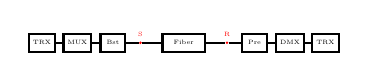
\begin{tikzpicture}[scale=0.25, every node/.style={scale=0.45}, line/.style={draw, thick}]
\node[draw, thick, minimum width=0.7cm, minimum height=0.5cm, font=\tiny] (tx) at (0,0) {TRX};
\node[draw, thick, minimum width=0.7cm, minimum height=0.5cm, font=\tiny] (mux) at (1.8,0) {MUX};
\node[draw, thick, minimum width=0.7cm, minimum height=0.5cm, font=\tiny] (boost) at (3.6,0) {Bst};
\node[circle, fill=red, inner sep=0.8pt] (s) at (5,0) {};
\node[font=\tiny, red] at (5,0.45) {S};
\node[draw, thick, minimum width=1.2cm, minimum height=0.5cm, font=\tiny] (fiber) at (7.2,0) {Fiber};
\node[circle, fill=red, inner sep=0.8pt] (r) at (9.4,0) {};
\node[font=\tiny, red] at (9.4,0.45) {R};
\node[draw, thick, minimum width=0.7cm, minimum height=0.5cm, font=\tiny] (preamp) at (10.8,0) {Pre};
\node[draw, thick, minimum width=0.7cm, minimum height=0.5cm, font=\tiny] (demux) at (12.6,0) {DMX};
\node[draw, thick, minimum width=0.7cm, minimum height=0.5cm, font=\tiny] (rx) at (14.4,0) {TRX};
\draw[line] (tx) -- (mux) -- (boost) -- (s) -- (fiber) -- (r) -- (preamp) -- (demux) -- (rx);
\end{tikzpicture}
\end{center}
\vspace{-4pt}
Budget: $P_{ch,S}-P_{ch,R}-L_{patch}$ • Unamp link

\section*{CONVERSIONS \& VALUES}

\subsection*{dB ↔ Linear}
$X_{dB} = 10\log(X)$ • $X = 10^{X_{dB}/10}$ • $P_{dBW} = P_{dBm} - 30$

3dB=$\times$2, 10dB=$\times$10, 20dB=$\times$100, 1dB=$\times$1.26, 6dB=$\times$4

\subsection*{Freq ↔ Wavelength}
$\lambda = c/f$, $c = 3 \times 10^8$ m/s • C-band: 1530-1565nm $\leftrightarrow$ 191-196THz

ITU-T: 100GHz=0.8nm, 50GHz=0.4nm, 12.5GHz=0.1nm @ 1550nm

\subsection*{Frequency Bands}
\textbf{RF:} L 1-2GHz, S 2-4, C 4-8, X 8-12, Ku 12-18, K 18-27, Ka 27-40, V 40-75, E 71-86, W 75-110
\textbf{Optical:} O 1260-1360nm, E 1360-1460, S 1460-1530, C 1530-1565, L 1565-1625
\textbf{Sat:} C-band 4/6GHz, Ku 11/14GHz, Ka 20/30GHz (down/up)

\subsection*{Logarithms}
$\log(2) = 0.301$ • $\log(3) = 0.477$ • $\ln(2) = 0.693$

\subsection*{Physical Constants}
$c = 3 \times 10^8$ m/s • $k = 1.38 \times 10^{-23}$ J/K • $h = 6.626 \times 10^{-34}$ J·s
$T_0 = 290$K (ref) • $\nu_{1550} = 194$THz • $1$ mW $= 0$ dBm $= -30$ dBW

\section*{EXAM STRATEGY}

\subsection*{RF Methodology}
(1) d (2) $A_{FSL}$ (units!) (3) G (4) EIRP (5) Loss (6) $P_R$ (7) N (8) C/N (9) Compare (10) Margin $\geq$2dB

\subsection*{Optical Methodology}
Unamp: $L_{max} = (P_{TX}-P_{RX,sens}-L_{conn}-L_{MUX})/\alpha$
Amp: (1) $N_{amp}=L/D_{amp}$ (2) $N_{ch}$ (3) $P_{ch}$ (4) OSNR (5) Margin

\subsection*{Critical Checks}
Units: km/m(60dB!), GHz/MHz, dBm/dBW(30dB) • Friis: LINEAR! • OSNR in 12.5GHz

Mistakes: $10\log(N_{amp})$, $B_{ch} \neq \Delta f$, Gain in dB, Wrong constant, PA BO, $T_A$

\subsection*{Sanity Checks}
\textbf{RF:} 40km@30GHz: $A_{FSL}\approx$125dB • LEO 1500km: 170dB • GEO: 200-210dB
1m@10GHz: G$\approx$30dBi • 1m@30GHz: 40dBi • Ant $\theta_{3dB}$: 1-100°
\textbf{Optical:} 100km loss: 18-20dB • EDFA: G=15-25dB, F=4-6dB
OSNR 1000km DP-QPSK: 15-18dB • TX: -3 to +3dBm • RX: -15 to -25dBm
\textbf{Typical:} Metro <100km, Regional 100-500km, Long-haul >500km

\subsection*{Formula Selection}
Distance+freq→$P_R$? Friis+link budget • Max distance? Solve for A

Minimize noise? Friis, LNA first • Multi-hop C/N? $1/(C/N)_{tot}=\sum 1/(C/N)_i$

Optical OSNR? $P_{ch}-F-58-10\log(N_{amp})$ • Modulation? Compare with threshold+margin

\end{multicols}

\end{document}
